% Focused research manuscript. No submission or editorial decision is implied.
% Uses the unchanged official PVLDB template pinned by build_vldb.py.
\documentclass[sigconf,nonacm]{acmart}
%%% VLDB block start %%%
\usepackage{pvldb}
%%% VLDB block end %%%
\renewcommand\vldbdoi{XX.XX/XXX.XX}
\renewcommand\vldbpages{XXX-XXX}
\renewcommand\vldbavailabilityurl{https://github.com/mandu5/sparse-vus/tree/research/saturation-20261021}
\newtheorem{theorem}{Theorem}
\newtheorem{lemma}{Lemma}
\newtheorem{proposition}{Proposition}
\newtheorem{corollary}{Corollary}
\newcommand{\ind}{\mathbf{1}}
\newcommand{\TP}{\mathrm{TP}}
\newcommand{\TPR}{\mathrm{TPR}}
\newcommand{\FPR}{\mathrm{FPR}}
\emergencystretch=2em
\begin{document}
\title{Active-Prefix Evaluation of Dynamic VUS}
\subtitle{Research manuscript}
\author{Youngmin Ko}
\email{rhdudals0505@naver.com}
\affiliation{\institution{Independent Researcher}\country{Republic of Korea}}
\begin{abstract}
Volume Under the Surface (VUS) evaluates time-series anomaly scores over
thresholds and tolerance widths. Existing support sweeps can still inspect
every maximum-support position at every width, even after the integral can
no longer change. We give an instance-sensitive evaluator for the original
dynamic-denominator, sum-and-clip VUS definition. A complete score threshold
permanently saturates recall when admitted original positives plus half the
admitted buffer mass reach the original positive count and every expanded
component has been hit. Its remaining PR contribution vanishes; its ROC
suffix telescopes analytically. Combining this condition with reversible
support activation and incremental component unions eliminates width-wise
full-support preparation. Under fixed-binary64 ranking and unit-cost metric
arithmetic, the full call takes
$O(n+L+\alpha(K)\sum_{w=0}^{L}J_w)$ time and $O(n+Q)$ auxiliary words,
where $J_w$ includes the complete terminating active score tie.
With one original interval and distinct support scores, the bound is
$O(n+LP_0)$ for every score ordering. For a singleton and $L\le n$, it
matches a deterministic score-query lower bound, giving optimal linear time
under the stated model. We evaluate 378 development cases on macOS and 144
external cases on each of macOS and Linux. The predeclared width-30 runtime
criterion fails in all three runs. At width 300, external median speedups
over the preceding sparse radix evaluator are $1.51\times$ and $1.63\times$,
with all 48 cases faster on each platform. Maximum observed PR discrepancy
in these three runs is below $3.67\times10^{-15}$.

Exactness refers to the mathematical all-threshold, all-width target;
floating-point parity and runtime are evaluated separately.
\end{abstract}
\maketitle
%%% VLDB block start %%%
\vldbtopmatter
%%% VLDB block end %%%
\section{Introduction}
Large anomaly-detection studies evaluate many score vectors against the same
time-series labels. VUS integrates a range-aware precision--recall or ROC
curve over tolerance widths, making evaluation itself a repeated analytics
operation~\cite{paparrizos2022,boniol2025}. Efficient exact evaluation matters
when an analyst wants exhaustive thresholds and every integer width rather
than a sampled approximation. We study the evaluator after scores have been
produced; detector training, inference, and data ingestion are separate costs.

Support restriction is already established in optimized VUS, and released
fast-VUS combines support-score sorting with cumulative
sums~\cite{boniol2025,klein2026}. Our earlier public Sparse VUS implementation~\cite{sparsevus03}
compresses negative-only threshold runs and uses binary64 radix preparation,
but still performs maximum-support work at every width. A full-recall cutoff
alone does not remove that preparation. We instead organize the computation
around the active score prefix whose contribution can change the answer.

Three features of the original metric make this nontrivial. First, its
positive and negative denominators depend on which buffer points pass the
threshold. Second, a separate existence factor rewards coverage of expanded
anomaly components, which merge as width increases. Third, points with zero
weight can share scores with active positions; removing them from a traversal
must not split a global tie or change precision and false-positive counts.

We address these features jointly. Complete global tie counts preserve the
effects of omitted positions. An offline reversible-list schedule activates
support positions in score order as widths increase. Incremental union-find
tracks component merges. The threshold scan stops only after both a mass
condition and complete component coverage permanently saturate recall. The
resulting bound depends on the actual visited prefix, without a hidden
width-by-support preprocessing term. A separating family establishes a
quadratic-to-linear traversal gap even against the same active-list method
stopped at the last original positive. A stronger single-interval guarantee
does not require a favorable score ordering, provided active scores are
distinct after conversion.

The study separates these mathematical claims from practical efficiency.
Whole-call timings include validation and preparation; matched ablations
disable saturation or retain only last-positive stopping. A predeclared
development corpus and a newly assembled external corpus test full-call
performance, numerical parity, and failure cases. These experiments measure
metric evaluation, not detector quality or complete model-selection pipelines.

\section{Target and exact event representation}
Let $y\in\{0,1\}^n$ contain both classes and $s\in\mathbb{R}^n$ contain finite
scores after binary64 conversion. Larger scores indicate greater anomaly
evidence. Let $P_0=\sum_i y_i$, and let the $K$ maximal original anomaly
intervals have inclusive endpoints $[a_k,b_k]$ in temporal order. Widths are
the integers $w=0,\ldots,L$. The continuous label $a_i^{(w)}$ is one on
original positives. An interval contributes $\sqrt{1-d/w}$ outside its
endpoints at integer distance $1\le d\le\lfloor w/2\rfloor$; contributions
are summed and clipped at one. At $w=0$ no ramp is added. Expanded intervals
that overlap merge, while adjacent nonoverlapping intervals remain separate.
This is the original dynamic VUS target pinned to the official
\texttt{RangeAUC\_volume\_opt} source at revision
\texttt{467bace0}, configured for exhaustive thresholds~\cite{vusreference}.
It is not shared by all software named VUS.

For a threshold $t$, define
\begin{align}
 p_i(t)&=\ind\{s_i\ge t\}, & C(t)&=\sum_i p_i(t),\\
 A(t)&=\sum_i y_i p_i(t), &
 B(t)&=\sum_i(1-y_i)a_i^{(w)}p_i(t),\\
 T(t)&=A(t)+B(t), & P(t)&=P_0+B(t)/2,\\
 N(t)&=n-P(t).
\end{align}
Let $H(t)$ count expanded components hit by at least one predicted positive,
and let $K_w$ count those components. The curve coordinates are
\begin{align}
 R(t)&=\min\{T(t)/P(t),1\}\,H(t)/K_w,\\
 F(t)&=(C(t)-T(t))/N(t), & \pi(t)&=T(t)/C(t).
\end{align}
Precision is used only at nonempty retained thresholds, where $C(t)>0$;
the initial origin requires no precision value.
The denominator is positive: $P(t)\le(n+P_0)/2<n$. ROC integrates trapezoids
from the origin through complete distinct descending score thresholds to
the explicit terminal $(1,1)$. PR uses the right-step sum
$\sum_j(R_j-R_{j-1})\pi_j$, with $R_0=0$. Each VUS scalar is the arithmetic
mean over every width. Signed horizontal ROC increments are preserved; the
derivation does not replace a dynamic denominator by a fixed one.

Let $S_w=\{i:a_i^{(w)}>0\}$, $Q_w=|S_w|$, and $Q=Q_L$. For an active event
with score $v_j$, precompute the complete global counts
$c_j^>=|\{i:s_i>v_j\}|$ and $c_j^\ge=|\{i:s_i\ge v_j\}|$. They include
positions outside $S_w$ and outside $S_L$.

\begin{lemma}[Inactive threshold runs]
Between consecutive active score events at a fixed width, $T,B,P,N,H,R$
are constant. Omitted thresholds contribute a horizontal ROC rectangle and
zero PR area. At an active score, its complete global numerical tie is a
single transition.
\end{lemma}
\begin{proof}
A newly admitted inactive point has zero weight and cannot hit an expanded
component. Only $C$ changes. The horizontal increments
$(\Delta C)/N$ telescope at fixed height $R$. All positions tied with an
active event enter at its global threshold, so both counts must retain them.
\end{proof}

If the previous retained state is $(T_o,N_o,R_o,c_o)$, event $j$ contributes
\begin{align}
 f_j^-&=(c_j^>-T_o)/N_o,\\
 \Delta\mathrm{ROC}_j&=
 (c_j^>-c_o)R_o/N_o+(F_j-f_j^-)(R_j+R_o)/2,\\
 \Delta\mathrm{PR}_j&=(R_j-R_o)T_j/c_j^\ge.
\end{align}
The initial state is $(0,n-P_0,0,0)$, and afterwards $c_o=c_j^\ge$.
Connecting retained endpoints without the intervening rectangle is
incorrect. For example, $y=(1,0,1,0)$, $s=(3,2,1,0)$ and $L=0$ give ROC
area $0.625$; connecting support endpoints alone gives $0.8125$.

\begin{lemma}[Two-distance geometry]
The weight of a non-original point is determined by its distances $d_1,d_2$
to the nearest two distinct original intervals. It is zero if
$d_1>\lfloor w/2\rfloor$, one if $d_2\le\lfloor w/2\rfloor$, and
$\sqrt{1-d_1/w}$ otherwise.
\end{lemma}
\begin{proof}
Every active ramp has weight at least $1/\sqrt2$. Two contributions therefore
clip to one. If exactly one interval contributes, its distance determines
the weight. Distances to ordered intervals are monotone moving away on each
side, so two neighbors on each side contain the nearest two intervals.
\end{proof}

\begin{proposition}[Fixed-binary64 preparation]
\label{prop:radix}
For finite binary64 scores, complete global tie counts, the score ordering
of maximum support, and its two-distance geometry can be prepared in
$O(n+Q+K)$ time and $O(n+Q)$ auxiliary words. Discrete work uses a word-RAM
with input indices, counts, widths, and intermediate index arithmetic
fitting words. Metric arithmetic, including square roots, has unit cost.
\end{proposition}
\begin{proof}
Normalize signed zeros. Complement a negative score's bit pattern and flip
the sign bit of a nonnegative score, then complement the result to obtain a
descending numerical key. Eight stable byte-counting passes order these
64-bit keys in $O(n)$ time. Scan complete ties and retain their starting and
ending global ranks. Filter the permutation to maximum-support positions.
A temporal scan with a monotone interval pointer computes nearest distances
and owners in $O(Q+K)$ time. All arrays are input- or support-sized.
\end{proof}
Radix sorting and floating-point key transforms are established
techniques~\cite{demaine2011radix,herf2001radix}. This assumption does not give
linear sorting of arbitrary real scores or a bit-complexity bound for growing
precision. Conversion defines numerical ties, including collisions between
distinct large integer inputs.

\section{Active-prefix algorithm}
\begin{figure}[t]
\begin{minipage}{\linewidth}
\textbf{Preparation (once).} Rank all scores; retain global tie counts.
Compute support distances and interval owners. Schedule activations and
component unions. Record insertion neighbors by reverse deletions.\\[3pt]
\textbf{For each width $w=0,\ldots,L$:}\\
1. Restore newly active positions and union newly overlapping intervals.\\
2. Set mass, hits and area to zero; start at the active list's head.\\
3. Visit the next complete active score tie; update mass and stamped hits.\\
4. Integrate its negative rectangle and global tied transition.\\
5. If $A+B/2\ge P_0$ and $H=K_w$, add ROC tail $1-F$ and finish the width.\\
6. Otherwise continue at step 3. Accumulate the width's scalar areas.\\[3pt]
\textbf{Return} the two means, or PR alone with ROC arithmetic omitted.
\end{minipage}
\caption{Active-prefix evaluation. Preparation occurs once. Each width visits
only its prefix and does not clear a support-sized or component-sized array.}
\Description{Preparation ranks scores and schedules activations. A width loop
restores active positions, merges components, then scans complete ties until
mass and component coverage saturate recall.}
\label{fig:active-algorithm}
\end{figure}
\subsection{Exact evaluation of active score prefixes}
\label{sec:saturation}
At a fixed width, let $A$ count admitted original-positive positions and let
$B$ denote their admitted non-original buffer mass. Then $T=A+B$ and
$P=P_0+B/2$. We call a complete score threshold \emph{saturated} when
\begin{equation}
 A+B/2\ge P_0\qquad\hbox{and}\qquad H=K_w.
 \label{eq:saturation-condition}
\end{equation}
The condition includes the complete global numerical tie, even when only some
positions in that tie belong to the width's active support.

\begin{lemma}[Permanent saturation]
After a threshold satisfying~\eqref{eq:saturation-condition}, every subsequent
recall coordinate equals one. The remaining right-step PR contribution is
zero, and the remaining trapezoidal ROC contribution, including the explicit
terminal $(1,1)$ transition, is $1-F$, where $F$ is the current FPR.
\end{lemma}
\begin{proof}
Threshold relaxation cannot decrease $A$, $B$, or the number of hit expanded
components. Thus both conditions persist. The first is equivalent to
$(A+B)/(P_0+B/2)\ge1$; the second makes the existence factor one. Every later
PR recall increment vanishes. Every later ROC trapezoid has height one, so
its signed horizontal increments telescope from the current $F$ to the
terminal abscissa one. The proof does not assume a fixed negative denominator.
\end{proof}

Stopping at recall one is a standard flat-curve observation, not a claimed
new integration principle. In particular, admitting the last original
positive gives $A=P_0$ and hits every expanded component, so it is already a
valid cutoff. The VUS-specific condition can stop earlier: buffer mass can
compensate for original positives that have not yet been admitted. Both
last-original-positive stopping and disabled stopping are explicit controls.

A cutoff added after constructing every width's full support histogram would
still pay $\Theta(Q)$ per width. To avoid that work, retain support positions
in descending score order, and activate position $i$ at radius $d_1(i)$;
original positives have activation radius zero. The score-ordered list is
represented by integer next pointers. Bucket-sort activations by their
integer radius. Starting from the full list, delete positions in reverse
activation order and record the two neighbors at each deletion. Reversing
these deletions inserts every position in constant time. Tied activation
radii use the same fixed order in both directions. Consequently traversing
the current list visits only positions with nonzero weight at that width.
A complete retained event still uses its precomputed global $c^>,c^\ge$;
points omitted from the current list may belong to that same global tie.

For geometry, preprocessing also records one nearest original interval for
each support position. At radius $r$, neighboring original intervals with
endpoints $b_k,a_{k+1}$ merge precisely when
$2r\ge a_{k+1}-b_k$. Bucket these edges by
$\lceil(a_{k+1}-b_k)/2\rceil$ and maintain their components with union-find.
Mere adjacency of expanded intervals does not merge them. An active point
lies in its nearest interval's expansion. Any other expansion containing the
point overlaps that expansion and belongs to the same component; hence the
nearest interval's union-find root identifies the point's component. A
width-stamped root array counts first hits without clearing all components
at each width. Unions occur before a width's threshold scan, so roots are
fixed throughout that scan.

\begin{theorem}[Active-prefix bound]
Use the fixed-binary64 word-RAM and unit-cost metric-arithmetic assumptions
of Proposition~\ref{prop:radix}. Let $J_w$ be the number of active support
positions visited through the complete first saturated score tie at width
$w$, and let $K$ count original intervals. Both scalar integrals can be
computed in
\[
 O\!\left(n+L+\alpha(K)\sum_{w=0}^{L}J_w\right)
\]
time and $O(n+Q)$ auxiliary words, where $\alpha$ denotes the inverse
Ackermann factor for union-find. A diagnostic vector of per-width work
counts uses an additional $O(L)$ words. The values equal the target
integrals in exact metric arithmetic.
\end{theorem}
\begin{proof}
Fixed-width radix ranking, complete global tie counts, the nearest-interval
scan, and extraction of the ordered support take $O(n+Q+K)$ time.
All activation distances and finite merge radii are at most $n-1$, so
bucket arrays are capped at $\min(\lfloor L/2\rfloor,n-1)+1$, even if $L$
is much larger than $n$. Counting-sort schedules and reverse deletions take
$O(n+Q+K)$ time and space. Each position is activated once, and there are
at most $K-1$ unions. Union by size with path compression takes amortized
$O(\alpha(K))$ per operation. Every visited position performs one find;
event arithmetic and first-hit accounting take constant additional time.
No width requires an additional $Q$- or $K$-sized scan. Streaming the means
requires $L+1$ width iterations. Since at width zero saturation requires all
original positives, $J_0=P_0\ge K$, and the union cost is absorbed by
$\alpha(K)\sum_w J_w$. Active-event elimination uses the same negative-run
rectangles as before, and the lemma supplies the exact omitted suffix.
All scratch state is input-, support-, or interval-sized.
\end{proof}

The bound is adaptive, not a worst-case improvement for every score vector:
$J_w$ may equal the full active support size. Union-find and linked-list
access also have costs that a work-count reduction does not measure.
Nevertheless, a separating family exists even against the same active-list
algorithm stopped at the last original positive. For $L\ge2$, take
$n=4L+3$, with singleton originals at zero-based positions $L+1$ and $3L+1$.
Rank first the first original, then its two immediate neighbors, then one
immediate neighbor of the second original. Rank the second original last;
put all remaining scores strictly between the fourth and last scores.
At every width $w\ge2$, those three neighbors have weight at least
$1/\sqrt2$, so the first four active positions satisfy
\[
 A+B/2\ge 1+\frac{3}{2\sqrt2}>2=P_0
\]
and hit both expanded components. Thus $J_w=4$, while at widths zero and
one $J_w=2$. The last-original-positive control must traverse
$Q_w=4\lfloor w/2\rfloor+2$ active positions at every width, giving
$\Theta(L^2)$ traversal rather than $\Theta(L)$. With $K=2$ and $n=\Theta(L)$,
the full adaptive algorithm takes $O(n+L)$ on this family. This is a
structural operation-count separation, not an empirical runtime claim.

The implementation uses finite-precision arithmetic and can differ from a
full scan through summation order and suffix telescoping. The theorem is an
exact-arithmetic identity; measured numerical parity, floating-point limits,
and runtime comparisons must be reported separately.

\subsection{A uniform mass bound for active prefixes}
\label{sec:saturation-mass-bound}
Let $S_w$ be the union of the expanded intervals at width $w$, and write
$Q_w=|S_w|$. List these active positions in decreasing score order, breaking
numerical ties arbitrarily but consistently. Numerical equality here is
that of the validated binary64 scores, including ties created by input
conversion. Only ends of complete active-score ties are valid event indices;
write their positive prefix lengths as
\[
 0=b_0<b_1<\cdots<b_g=Q_w.
\]
For $1\le q\le Q_w$, define the tie-rounding map
\[
 \rho_w(q)=\min\{b_j:b_j\ge q\}.
\]
Global positions outside $S_w$ may share these scores. They remain included
in the event's global prediction count, but are not counted in $Q_w$ or $b_j$.

\begin{lemma}[Active support and prefix mass]
For the stated half-width square-root ramps, $S_w$ is precisely the set of
positions with positive label weight and precisely the set of positions
capable of hitting an expanded component. Every active original position
contributes one to $A+B/2$; every active non-original position contributes
at least $1/(2\sqrt2)$. Therefore, after any $q$ active positions have been
admitted, even within a score tie,
\[
 A+B/2\ge q/(2\sqrt2).
\]
\end{lemma}
\begin{proof}
At widths zero and one the active positions are exactly the originals, each
of weight one. At width $w\ge2$, a non-original position is in $S_w$ exactly
when at least one original interval is at integer distance
$d\le\lfloor w/2\rfloor$. Its contribution from that interval is
$\sqrt{1-d/w}\ge1/\sqrt2$. Summing additional nonnegative contributions
and clipping at one preserves this lower bound. Such a position contributes
half its weight to $A+B/2$, while an original contributes one. Summing gives
the inequality. The same union defines expanded-component membership, so
positions outside $S_w$ cannot change either mass or component hits.
\end{proof}

Let $M_w$ be the first complete active-event prefix length with
$A+B/2\ge P_0$, and let $E_w$ be the first complete active-event prefix
length that hits all $K_w$ expanded components. Both exist: at $b_g=Q_w$,
all originals have been admitted, so $A=P_0$, and every expanded component
contains an admitted original. Put
\[
 m=\lceil2\sqrt2 P_0\rceil.
\]

\begin{proposition}[Mass and coverage bound with complete ties]
For the evaluator stopped at the first mass-and-coverage saturation event,
\begin{align}
 J_w&=\max\{M_w,E_w\},\\
 M_w&\le\rho_w(\min\{Q_w,m\}),\\
 J_w&\le\rho_w\!\left(\min\{Q_w,\max\{E_w,m\}\}\right).
 \label{eq:mass-coverage-bound}
\end{align}
If $\tau_w=\max_j(b_j-b_{j-1})$ is the largest active-score tie size, then
\[
 J_w\le\min\{Q_w,\max\{E_w,m+\tau_w-1\}\}.
\]
\end{proposition}
\begin{proof}
Mass and coverage are each nondecreasing under threshold relaxation.
Their first complete-event indices are $M_w$ and $E_w$, so both conditions
first hold at their maximum. If $Q_w\ge m$, the preceding lemma guarantees
the mass condition after $m$ positions; it still holds after completing
that tie. If $Q_w<m$, the final event contains every original and satisfies
the mass condition. This proves the bound on $M_w$. Since $E_w$ is already
a complete-event prefix length, taking its maximum with the rounded mass
bound gives~\eqref{eq:mass-coverage-bound}. Finally,
$\rho_w(q)\le\min\{Q_w,q+\tau_w-1\}$, which yields the stated additive-tie
bound. No partial tie is used as an evaluation threshold or stopping point.
\end{proof}

\begin{corollary}[One original interval]
If $K=1$ and the validated scores within $S_L$ are pairwise distinct, then
for every score ordering and every width,
\[
 J_w\le\min\{Q_w,\lceil2\sqrt2 P_0\rceil\}.
\]
Under the preceding computation model, the complete scalar evaluator takes
$O(n+(L+1)P_0)=O(n+LP_0)$ time and $O(n+Q)$ auxiliary words. In particular,
a single original anomalous position ($P_0=K=1$) gives $J_w\le3$ and total
$O(n+L)$ time, without a score-quality assumption. At widths zero and one,
$J_w=1$ in that singleton case.
\end{corollary}
\begin{proof}
There is one expanded component at every width. The first active position
hits it, and with distinct active scores $E_w=1$ and $\rho_w(q)=q$.
Apply the proposition. Union-find operations are constant time when $K=1$,
and sum the per-width bound. Since $P_0\le n$, the additional $P_0$ term is
absorbed into $O(n+LP_0)$. For $P_0=1$, $\lceil2\sqrt2\rceil=3$.
\end{proof}

The distinctness requirement concerns active/support scores, not arbitrary
off-support scores. Equal scores exclusively outside $S_L$, or off-support
positions tied with a single active position, do not enlarge an active tie.
More generally, with one original interval and $\tau_w\le\tau$ at every
width, the same analysis gives $O(n+(L+1)(P_0+\tau))$ time.

Arbitrary active ties prevent the singleton corollary for this
position-by-position evaluator. For $L\ge1$ and $n=2L+1$, place the only original at
zero-based position $L$ and assign all $n$ positions the same score. At
width $w$, the sole active event contains
$Q_w=2\lfloor w/2\rfloor+1$ positions. The evaluator visits that complete
event, so $J_w=Q_w$ and $\sum_{w=0}^L J_w=\Theta(L^2)$, although
$P_0=K=1$. This is a counterexample to dropping the tie restriction from
this evaluator's bound; it is not a lower bound for all possible VUS
algorithms or for implementations that aggregate tied masses differently.

For multiple original intervals, the mass bound alone does not bound the
coverage prefix $E_w$. A component whose active scores are all low can keep
$E_w$ near $Q_w$ even after the mass condition holds. Thus neither small
$P_0$ alone nor the mass inequality supplies a general multi-component
$O(n+LP_0)$ guarantee. The proof concerns the pinned ramp, denominator,
component-hit definition, and complete-threshold scalar target in exact
metric arithmetic; finite-precision stopping is numerically validated
separately.

\subsection{Linear input-inspection optimality for a singleton anomaly}
\label{sec:singleton-optimality}
The preceding upper bound admits a matching input-inspection lower bound
on a restricted class. The input-access model matters: an algorithm is
deterministic and adaptively reads individual score coordinates in random
access. Reading a coordinate reveals its validated binary64 value. The labels,
$n$, and $L$ may be supplied without charge, and validity and pairwise score
distinctness are promised. No precomputed ordering, score summary, or
certificate is supplied. A unit-time word operation reads at most a constant
number of score coordinates. Thus the argument does not charge input
validation and does not concern parallel or aggregate-query oracles.

\begin{theorem}[Singleton score-query lower bound]
\label{thm:singleton-query-lower}
Fix integers $n\ge4$ and $0\le L\le n$, and assume that the score domain
contains $n-1$ distinct finite binary64 values below one. Every deterministic
algorithm that exactly evaluates scalar VUS-PR on all inputs with these
$n,L$, one original anomalous position, and pairwise distinct validated
scores must, on some such input, inspect at least
\[
 n-\lfloor L/2\rfloor-1
 \;\ge\;\lceil n/2\rceil-1
 \;\ge\;n/4
\]
distinct score coordinates. The same lower bound applies when the requested
output is the pair VUS-ROC and VUS-PR.
\end{theorem}
\begin{proof}
Fix the label vector $y=(1,0,\ldots,0)$; the algorithm may know this vector
for free. Set $r=\lfloor L/2\rfloor$. Because the only original is at the
left boundary, its maximum support is $S_L=\{0,\ldots,r\}$. Let
$U=\{r+1,\ldots,n-1\}$, so $|U|=n-r-1$. Choose a base score vector with
$s_0=1$ and all other scores distinct and below one. For example,
$s_i=-i$ for $i\ge1$ is exactly representable when $n\le2^{53}$.
At every width $w\le L$, the first admitted position is the original:
$A=1$, $B=0$, $H=K_w=1$, and the prediction count is one. Recall jumps
from zero to one at precision one and remains one thereafter. Hence every
width has PR area one, and the scalar average is one.

Suppose the algorithm's execution on this base input terminates without
inspecting some $j\in U$. Change only $s_j$ to two. The modified input is
still finite and pairwise distinct. Since $j\notin S_L$, it is outside the
support and every expanded component at every $w\le L$. On the modified
input it is admitted first, with zero recall; the original is admitted
second, with $A=1$, $B=0$, $H=K_w=1$, and prediction count two. The only
nonzero recall increment is therefore from zero to one at precision
$1/2$. All later recall increments vanish. Every width has PR area $1/2$,
and so does their scalar average.

The two adaptive query transcripts are identical. Inductively, identical
previous query answers make a deterministic algorithm choose the same next
query or termination action; every queried coordinate has the same value
because coordinate $j$ was never read in the base execution. Consequently
the algorithm returns the same output on both inputs, contradicting their
different exact scalar PR values. It must therefore inspect every coordinate
in $U$ on the base input. Counting these coordinates gives the stated bound.
An algorithm returning both scalar integrals must return the PR component,
so the same adversary applies to that output pair.
\end{proof}

\begin{corollary}[Linear-time optimal singleton subclass]
\label{cor:singleton-linear-optimal}
Under the fixed-key word-RAM and unit-cost exact metric-arithmetic model,
for inputs with $P_0=K=1$, pairwise distinct validated binary64 scores,
and $0\le L\le n$, the active-prefix evaluator uses $O(n)$ time and
$O(n)$ auxiliary words, uniformly over anomaly locations and score
orderings. Its worst-case time order matches the deterministic
$\Omega(n)$ score-inspection lower bound for exact scalar VUS-PR and for
the pair of scalar VUS-ROC and VUS-PR.
\end{corollary}
\begin{proof}
The singleton mass bound gives $J_w\le3$ for every width. Preprocessing and
all width evaluations therefore take $O(n+L)=O(n)$ time; $Q\le n$ gives
the memory bound. The boundary-location inputs in
Theorem~\ref{thm:singleton-query-lower} belong to this subclass and require
at least $n/4$ score inspections. A constant number of such inspections per
word operation gives the matching worst-case time lower bound.
\end{proof}

The lower bound is a finite-instance query statement for feasible distinct
binary64 inputs; the explicit integer witness covers $4\le n\le2^{53}$.
The asymptotic notation uses the same fixed-key operation-count convention
as the upper bound, rather than asserting an unbounded sequence of distinct
values in a literally finite 64-bit universe. Input validity need not be
verified for the lower bound. No assumption promises that the original
has the highest score: that property holds only for the adversary's base
input. The conclusion is deterministic input-inspection optimality within
the stated singleton subclass. It gives no $\Omega(L)$ lower bound for
$L\gg n$, no general $\Omega(n+L)$ lower bound, no randomized lower bound,
and no firstness or practical-performance claim.


\subsection{Implementation and arithmetic contract}
The implementation supplies a PR-only public call and a paired ROC--PR call.
Both validate inputs, prepare ranking and geometry, and stream the mean over
widths. They use the same active-list kernel; the PR route omits ROC arithmetic.
Diagnostic profiles additionally return actual visited and active counts for
every width and are never included in metric timings. A disabled-stop control
visits the entire active list. A last-original-positive control has identical
preparation and component bookkeeping but stops only at $A=P_0$.

Active lists and interval unions are reused across widths, but area values
cannot generally be reused for consecutive odd and even widths. Although
$\lfloor w/2\rfloor$ can be equal, the ramp $\sqrt{1-d/w}$ changes. For
$y=(0,1,0)$ and $s=(2,1,0)$, width-two PR is about $0.77705$, whereas
width-three PR is about $0.85505$. Every integer width is therefore evaluated.

The proofs describe exact metric arithmetic. Compiled implementations use
finite precision without a claim of symbolic or bitwise identity. Summation
order, square roots, and suffix telescoping can change final bits. Rounding
can also change the saturation predicate; no directed-rounding certificate
or all-input floating-point error bound is claimed. Testing
therefore compares scalar values against separately constructed references,
and timing decisions require the frozen numerical tolerance on every case.

\section{Related work}
Original VUS and its optimized implementations motivate restricting label
work to maximum buffers~\cite{paparrizos2022,boniol2025}. Klein's released
fast-VUS sorts support scores and uses cumulative sums at each width; it is
the closest inspected external PR-only implementation~\cite{klein2026}.
Our public version 0.3~\cite{sparsevus03} supplies support events, two-distance geometry and
radix execution, and is an explicit baseline here. The present contribution
is the active-prefix computation and its bounds, not those earlier
ingredients by themselves.

Sorted curve scans, complete ties and trapezoidal integration are standard
ROC techniques~\cite{fawcett2006}. The scikit-learn 1.0.2 PR routine explicitly
truncates its returned curve at full recall after constructing cumulative
counts~\cite{sklearn102}. Thus the observation that recall-one suffixes add
no PR area is established. Last-positive stopping is a necessary control.
Our mass condition can stop before the last original positive, and its
benefit is realized only when preparation also avoids full-support work.

Reverse deletion and restoration follow the established reversible-list
technique described by Knuth~\cite{knuth2000}. The union-find implementation
uses union by size and path halving, whose amortized analysis is established
by Tarjan and van Leeuwen~\cite{tarjan1984}. Our complexity proof accounts
for how often this problem invokes those operations; it does not introduce
a new list or disjoint-set data structure.

Sylligardos reports preliminary CPU and GPU VUS acceleration in a Ph.D.
workshop paper~\cite{sylligardos2025}. Public Sylligardos-attributed FF-VUS
code exists in aVUSi~\cite{ffvus2026}. Its native geometry and integration
contract differ from the original target used here, and the wrapper rounds
scores. We retain this relevant prior work without interpreting its native
runtime as an exact-target comparison. Similarly, package names alone do not
establish semantic equivalence. Source revisions and concrete semantic
witnesses are included with the artifact. The bounds and measurements here
do not establish superiority over an unmeasured GPU implementation.

\section{Experimental design}
The primary task is one exact PR scalar for a fixed label vector, score
vector and maximum width. Every method receives identical arrays in a case.
The candidate, both stopping ablations, version-0.3 sparse radix, matched
nearest-distance dense radix, actual pinned Klein fast-VUS, sparse comparison
sorting, direct dense comparison sorting and direct dense radix form nine
methods. All are PR-only in this study; Klein receives $n$ thresholds to
evaluate the exhaustive target. The other evaluators process distinct global
ties. Repeated tied thresholds in Klein add zero recall increments.

The development set contains 42 previously studied series and three released
foundation-model score vectors per series~\cite{zhu2026}. It is not an unseen
corpus. The external set was selected from mTSBench metadata before scores
or metric outcomes were computed~\cite{mtsbench}. We excluded the 23 earlier
source-family names with recorded alias normalization, restricted test
lengths to at most 100,000, and selected the lexicographically first two
eligible series per family. This yields 12 series from nine source families,
457,171 rows in total. Source-family disjointness does not prove independent
real-world domains. GutenTAG synthetic data and reused source
datasets are identified in the manifest.

Four label-free CPU scoring procedures generate the external inputs:
Isolation Forest, standardized PCA reconstruction error, reference-set
nearest-neighbor distance, and robust marginal deviation. Their preprocessing,
seeds and parameters were fixed before metric evaluation. These are diverse
score inputs, not claims of anomaly-detection quality or reproductions of a
benchmark's detector pipeline. Model generation is outside the timed metric
calls. Raw and derived array hashes bind every case.

Maximum width 30 is primary; 100 and 300 are secondary and stress conditions.
Thus development has 378 series--model--width cases, while external
confirmation has 144; the primary external width contains 48 score vectors
from 12 series, not 144 independent datasets. Each case has three warmed,
serial, complete-call timing repetitions in a seeded randomized method order.
Validation, score conversion, sorting and all preparation are timed. Data I/O,
imports, JIT warm-up and diagnostic profiles are excluded. Compute libraries
and Numba use one thread. Source and input hashes are frozen before each
run, and all losses are retained. Environment and process snapshots are
recorded; the local host is not a dedicated isolated benchmark machine.
The Mac runs use an Apple M1 Pro with Python 3.12.4. The hosted Ubuntu
24.04 runner reports an AMD EPYC 9V74 processor, four exposed logical CPUs,
and Python 3.12.15. Both use NumPy 1.26.4 and Numba 0.59.1. Measurements
use one compute thread on each host; host and background-load effects are
not experimentally separated.

The predeclared primary criterion requires maximum absolute discrepancy at
most $10^{-11}$ on all cases and lower 95\% family-cluster bootstrap bounds
above one for both geometric and aggregate speed ratios against each of the
eight controls at width 30. Ratios are control time divided by candidate
time. We pair medians within a run and resample source families 2,000 times.
These intervals characterize the observed family/case variation, not
timing-repeat uncertainty, unseen machines, or the population of all domains.
Aggregate ratios compare sums of per-case medians. Passing this criterion
supports the stated experiment; it does not establish global firstness.

\section{Results}
\subsection{Numerical agreement and primary decision}
All 666 cases across the three main runs meet the frozen $10^{-11}$ PR
tolerance. Maximum absolute discrepancy is $1.34\times10^{-15}$ on Mac
development and $3.67\times10^{-15}$ on each external run, rounded upward.
An additional independently written dense oracle constructs ramps, expanded
components, complete global thresholds and both integrals without calling
the production geometry or integration helpers. Its 8,606 cases include
small exhaustive binary labels and tied scores, all widths through $2n+1$,
and noncontiguous inputs. Across 51,636 public calls, maximum discrepancy is
$3.34\times10^{-16}$ for the paired output and $2.23\times10^{-16}$ for
PR-only output, rounded upward. This is numerical evidence, not a proof of
correct rounding for arbitrary floating-point inputs.

\textbf{The predeclared primary runtime criterion fails in all three runs.}
At $L=30$, median ratios against released sparse radix are 1.016 on Mac
development, 1.026 on Mac external and 1.013 on Linux external, with
52/126, 19/48 and 21/48 candidate losses. The family-bootstrap criterion
does not hold against every matched control. A faster reference library
comparison cannot override these outcomes. Table~\ref{tab:saturation-all-controls}
retains all eight controls, all widths and the number of losses.
% Generated by experiments/render_saturation_paper_results.py; do not edit data by hand.
% Evidence SHA256: aa3eb2bfd095ba0f54cde12721f0254e04cdd2a7456ab2cb593e0ce8270a8b34
% Renderer SHA256: 189c745a0754b9b568b5a896991a351828668d57ab4b6238256e55103a520c14
% Independent auditor SHA256: 261303ab275b6afce8cfb1160955fd5f6bd88bfdd17b950e190eec39861ba4ab
\begin{table*}[t]
\centering
\footnotesize
\setlength{\tabcolsep}{2.5pt}
\renewcommand{\arraystretch}{1.10}
\begin{tabular}{l*{9}{r}}
\toprule
 & \multicolumn{3}{c}{Mac development} & \multicolumn{3}{c}{Mac external} & \multicolumn{3}{c}{Linux external} \\
\cmidrule(lr){2-4}\cmidrule(lr){5-7}\cmidrule(lr){8-10}
Control & $L=30$ & $L=100$ & $L=300$ & $L=30$ & $L=100$ & $L=300$ & $L=30$ & $L=100$ & $L=300$ \\
\midrule
Full active scan & 1.005(59) & 1.057(38) & 1.271(15) & 1.007(22) & 1.041(14) & 1.216(3) & 1.017(19) & 1.063(9) & 1.218(2) \\
Last-positive stop & 1.011(54) & 1.040(42) & 1.198(21) & 1.012(22) & 1.059(13) & 1.136(6) & 1.025(19) & 1.041(12) & 1.152(6) \\
Released radix & 1.016(52) & 1.191(14) & 1.660(1) & 1.026(19) & 1.151(2) & 1.506(0) & 1.013(21) & 1.202(3) & 1.627(0) \\
Dense nearest radix & 2.602(5) & 4.607(0) & 8.107(0) & 2.835(0) & 6.250(0) & 13.188(0) & 3.274(0) & 7.689(0) & 13.526(0) \\
fast-VUS & 20.175(0) & 41.291(0) & 72.435(0) & 16.908(0) & 42.627(0) & 92.597(0) & 13.174(0) & 28.616(0) & 57.738(0) \\
Sparse comparison sort & 2.041(9) & 2.087(6) & 2.285(0) & 1.783(5) & 1.816(5) & 1.997(4) & 1.630(9) & 1.678(8) & 1.993(8) \\
Dense direct & 3.286(3) & 5.518(0) & 10.557(0) & 3.478(0) & 6.401(0) & 13.643(0) & 3.657(0) & 8.412(0) & 14.453(0) \\
Dense direct radix & 2.672(5) & 4.970(0) & 10.124(0) & 3.008(0) & 6.218(0) & 13.439(0) & 3.023(0) & 7.705(0) & 14.128(0) \\
\midrule
Fastest eight-control oracle & 0.978(84) & 1.006(60) & 1.136(24) & 0.980(32) & 1.023(19) & 1.113(9) & 0.984(29) & 1.030(18) & 1.142(10) \\
\bottomrule
\end{tabular}
\caption{Median paired runtime ratio (control divided by saturation), with the number of slower saturation cases in parentheses. Cases per width: Mac development: 126; Mac external: 48; Linux external: 48. A ratio below one favors the control. Each case uses the median of three complete public-call timings. The oracle selects the fastest of the eight measured controls separately for each case, after measurement. All cases and widths are retained. Frozen primary $L=30$ criterion: Mac development: FAIL; Mac external: FAIL; Linux external: FAIL.}
\label{tab:saturation-all-controls}
\end{table*}


\subsection{Secondary widths and practical overhead}
At $L=300$, median ratios against released sparse radix are 1.660 on
development, 1.506 on Mac external and 1.627 on Linux external. The candidate
wins 125/126, 48/48 and 48/48 corresponding comparisons. The external
family-bootstrap intervals are [1.417, 2.634] and [1.527, 2.982] for the
geometric ratios, and [1.392, 2.472] and [1.554, 2.993] for aggregate ratios.
These are the prespecified secondary/stress widths; they do not replace
the failed primary test. Absolute sums of per-case median times at $L=300$
are 0.584 versus 0.914 seconds on Mac external and 0.738 versus 1.388 seconds
on Linux external for candidate versus released radix. These sums describe
48 separately timed calls and are not a measured end-to-end application.

To avoid selecting a weak comparator, we also report a post-measurement
oracle that chooses the fastest of the eight controls separately per case.
It is not a deployable selector. At $L=30$ its median ratios are below one
in all three runs. At $L=300$ they are 1.136, 1.113 and 1.142, with
24/126, 9/48 and 10/48 candidate losses. In particular, beating released
radix in every external stress case does not mean beating every measured
control. Figure~\ref{fig:saturation-cdf} shows the entire ratio distributions.

\begin{figure*}[t]
\centering
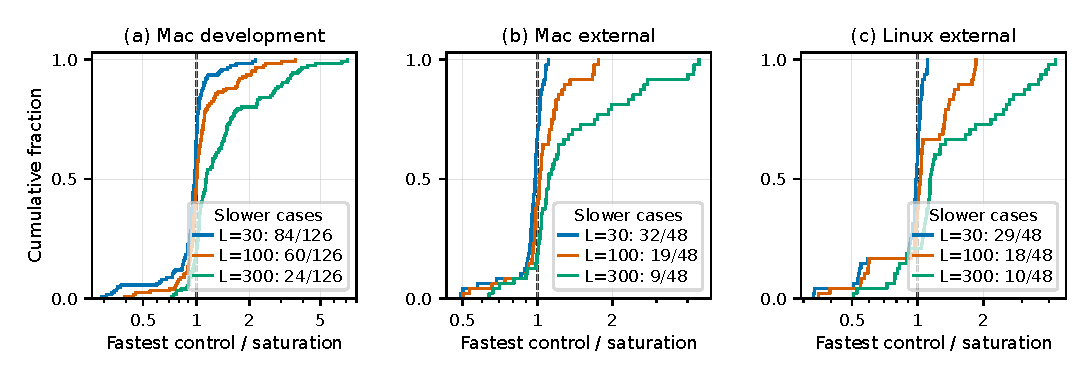
\includegraphics[width=\textwidth]{figures/saturation-cdf.pdf}
\caption{Whole-call speed ratios against the fastest measured control for
every case. The dashed line is equal runtime; values below one favor the
control. Each panel retains all three widths and reports the count of slower
candidate cases. Runs are summarized separately rather than pooled.}
\Description{Three cumulative-distribution panels for Mac development,
Mac external and Linux external, showing every width and slower-case count.}
\label{fig:saturation-cdf}
\end{figure*}

The work profiles explain a mechanism without equating work reduction with
speed. At $L=300$, aggregate saturation visits are 72.1\%, 57.5\% and
57.5\% of full-active visits, and 73.8\%, 58.3\% and 58.3\% of
last-positive visits, respectively. Median runtime ratios against the
last-positive control are 1.198, 1.136 and 1.152. Preparation, pointer
access and component bookkeeping still cost time; some cases with fewer
visits remain slower. Figure~\ref{fig:saturation-work} compares work and time
against the matched full-active control for every case; it is a descriptive
association, not an estimate of the causal cost of one visit. Seven development
series and four external series have one original interval. The theorem also
requires distinct support scores; interval count alone does not establish
its applicability.

\begin{figure*}[t]
\centering
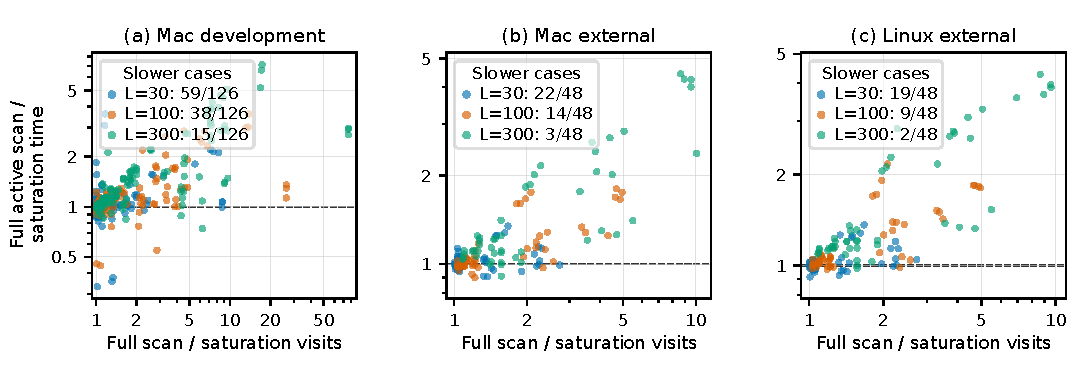
\includegraphics[width=\textwidth]{figures/saturation-work.pdf}
\caption{Traversal reduction versus full-call runtime. Horizontal position
is full-active visits divided by saturation visits; vertical position is
full-active time divided by saturation time. A work saving need
not cross the horizontal equal-runtime line. Every measured case is retained.}
\Description{Three scatter panels relate traversal reduction to complete-call
speed ratio for all cases and widths on the three study runs.}
\label{fig:saturation-work}
\end{figure*}

\subsection{Linux regeneration and additional external implementations}
The frozen Linux workflow regenerated the external inputs from pinned raw
sources, then ran the same protocol with the same source hashes. Raw data
and labels match Mac hashes. Eleven of 48 score arrays match byte for byte;
37 differ after platform-dependent scoring. This is a reproduction of the
specified input-generation procedure and evaluator experiment, not an
identical-array replay or an independent laboratory study. All 53 downloaded
artifact-file hashes were checked against the workflow manifest.

A separately frozen descriptive supplement compares the paired ROC--PR
public call against actual pinned Benchopt and DTAI implementations, with
exhaustive thresholds~\cite{benchopt2026,dtaianomaly}. It uses the 48 external
score vectors at $L=30$, three warmed complete-call repetitions, and the
released paired radix evaluator as a control. The native DTAI code retains
its parallel/fast-math compilation but runs with one compute thread.
Benchopt completes all 48 cases: its median ratio is $34.918\times$ and
the minimum is $20.079\times$. The paired radix median is only $1.017\times$,
with 19/48 candidate losses. Thus the large external-library ratio cannot
be attributed to saturation alone.

DTAI is prescribed for the Isolation Forest vector of each of the 12
series. Ten complete all repetitions; PSM and swan hit the 30-second parent
watchdog on their first timed call, and subsequent repetitions are skipped.
The two cases receive no fabricated evaluator duration or speed ratio.
The completed subset has median ratio $101.106\times$; censoring prevents
interpreting it as the median over all 12 prescribed cases. All completed
paired outputs agree within $8.22\times10^{-15}$. This supplement neither
changes the main experiment's task nor its primary decision.

\subsection{Structural mechanism checks}
A separately frozen synthetic study tests four input families at
$L\in\{32,128,512,2048\}$, with $n=4L+3$. The first places a singleton
original last among distinct scores; the second uses an eight-position
original interval with all originals last; the third realizes the
two-original separating construction, with equal middle scores below its
four decisive positions; the fourth is an all-tied singleton negative
control. All inputs, source hashes and count predictions are fixed before
timing. Each case uses three randomized warmed complete-call repetitions.
All 16 cases satisfy their count predictions and agree with released radix
within $1.39\times10^{-17}$. This comparison uses production radix rather
than an additional independent dense oracle.

The singleton distinct-score family visits $3L-1$ positions in total;
the two-original family visits $4L$. At $L=2048$, the latter visits 8,192
positions versus 4,198,402 for last-positive stopping, a $512.5\times$
traversal reduction. Its median full call takes 0.717 milliseconds, with
$17.06\times$ speedup over last-positive stopping and $53.88\times$ over
released radix. The all-tied singleton instead visits the entire active
support, as predicted. Its last-positive ratio remains close to one.
These constructed inputs demonstrate mechanisms and their limitations;
their timing gains do not estimate gains on real-world data.

\begin{table}[t]
\centering
\footnotesize
\setlength{\tabcolsep}{3.5pt}
\begin{tabular}{lrrrr}
\toprule
Family & $L=32$ & 128 & 512 & 2048\\
\midrule
Singleton, original last & 0.845 & 1.401 & 4.530 & 17.536\\
Eight originals last & 1.019 & 1.273 & 3.354 & 12.793\\
Two-original separation & 1.025 & 1.387 & 4.161 & 17.063\\
All-tied singleton & 0.972 & 1.005 & 0.998 & 1.012\\
\bottomrule
\end{tabular}
\caption{Descriptive structural-study ratios: last-positive median time
divided by saturation median time. All 16 cases are shown, including small
input overhead and the tied negative control.}
\label{tab:structural-runtime}
\end{table}



\section{Limitations and reproducibility}
The active-prefix bound is adaptive. Component coverage can require low-ranked
points, and a large terminating tie can force traversal of most active
support. Pointer access, union-find and preparation introduce overhead. A
reduction in visited positions therefore need not reduce full-call runtime.
The scalar algorithm does not return the entire threshold surface. Its
linear preparation assumes finite fixed-width binary64 keys; exact real
arithmetic in the theorem is distinct from implemented floating-point math.

The small external corpus was selected reproducibly but does not exhaust
anomaly-label geometries, score ties or source domains. Its four score
generators share simple CPU preprocessing, and no detector-quality claim is
made. Hardware conclusions are limited to the measured environments. GPU
acceleration and methods with different native VUS definitions require
separate fidelity and hardware comparisons.

The artifact contains the implementation, tests, theorem sources, independent
oracle, frozen protocols, append-only measurements, every slower case and
report reconstruction code. External data are downloaded from pinned public
sources and regenerated locally; the artifact does not relicense or bundle
raw third-party data. Source-specific data terms are recorded separately.
The Linux reproduction preserves raw/label identity and reports every score
hash match or difference instead of assuming bitwise cross-platform scores.

\paragraph{AI assistance disclosure.}
OpenAI Codex assisted with literature retrieval, algorithm and proof
development, implementation, experiment orchestration, testing, and manuscript
drafting. Separately prompted agent contexts constructed the oracle and
reviewed mathematical and empirical claims within the same workflow. These
checks are internal verification, not independent laboratory replication or
external peer review. The artifact records the generated code and measured
evidence; AI tools are not listed as authors.

\section{Conclusion}
Exact dynamic VUS can be evaluated by active score prefixes while accounting
analytically for omitted thresholds. Reversible activation and incremental
component unions remove the per-width maximum-support setup that would
otherwise hide behind a stopping rule. The resulting instance-sensitive bound,
the single-interval guarantee, and the separation from last-positive stopping
characterize when less traversal is possible. The empirical study separately
tests whether those savings survive complete-call costs.

\bibliographystyle{ACM-Reference-Format}
\bibliography{active_prefix_references}
\end{document}
